\section{Analysis of the Fault Model}
\label{sec:fault_analysis}

A  benefit of utilizing the AGREE behavioral annex is the ability to perform both monolithic and compositional analysis on the nominal model. AGREE allows {\em assume-guarantee} behavioral contracts to be added to AADL components.  The language used for contract specification is based on the Lustre dataflow language~\cite{Halbwachs91:IEEE} and the nominal model (AADL model annotated with AGREE contracts) is translated into Lustre before being sent to the JKind model checker for verification\cite{2017arXiv171201222G}. 

When a user selects to run the fault analysis during verification, the AGREE contracts are automatically extended in Lustre in order to allow faults to modify the behavior of component outputs. These injections into the Lustre model are shown in Figure~\ref{fig:lustre}. In the left column of the figure, the nominal Lustre pump definition is shown with an AGREE contract on the output. 

In the right column, the additional local variables for the fault are seen in boxes 1 and 2, the assertion binding the fault value to the nominal value is seen in boxes 3 and 4, and the fault node definition is given in box 5. To support these extensions, AGREE implements an Eclipse extension point interface that allows other plug-ins to modify the generated abstract syntax tree (AST) prior to its submission to the solver.  If the Safety Annex is enabled by the user, these faults are added to the Lustre model and, if triggered, override the nominal guarantees provided by the component.

\begin{figure}[h!]
	\hspace*{-2cm}
	\vspace{-0.3in} 
	\begin{center}
		%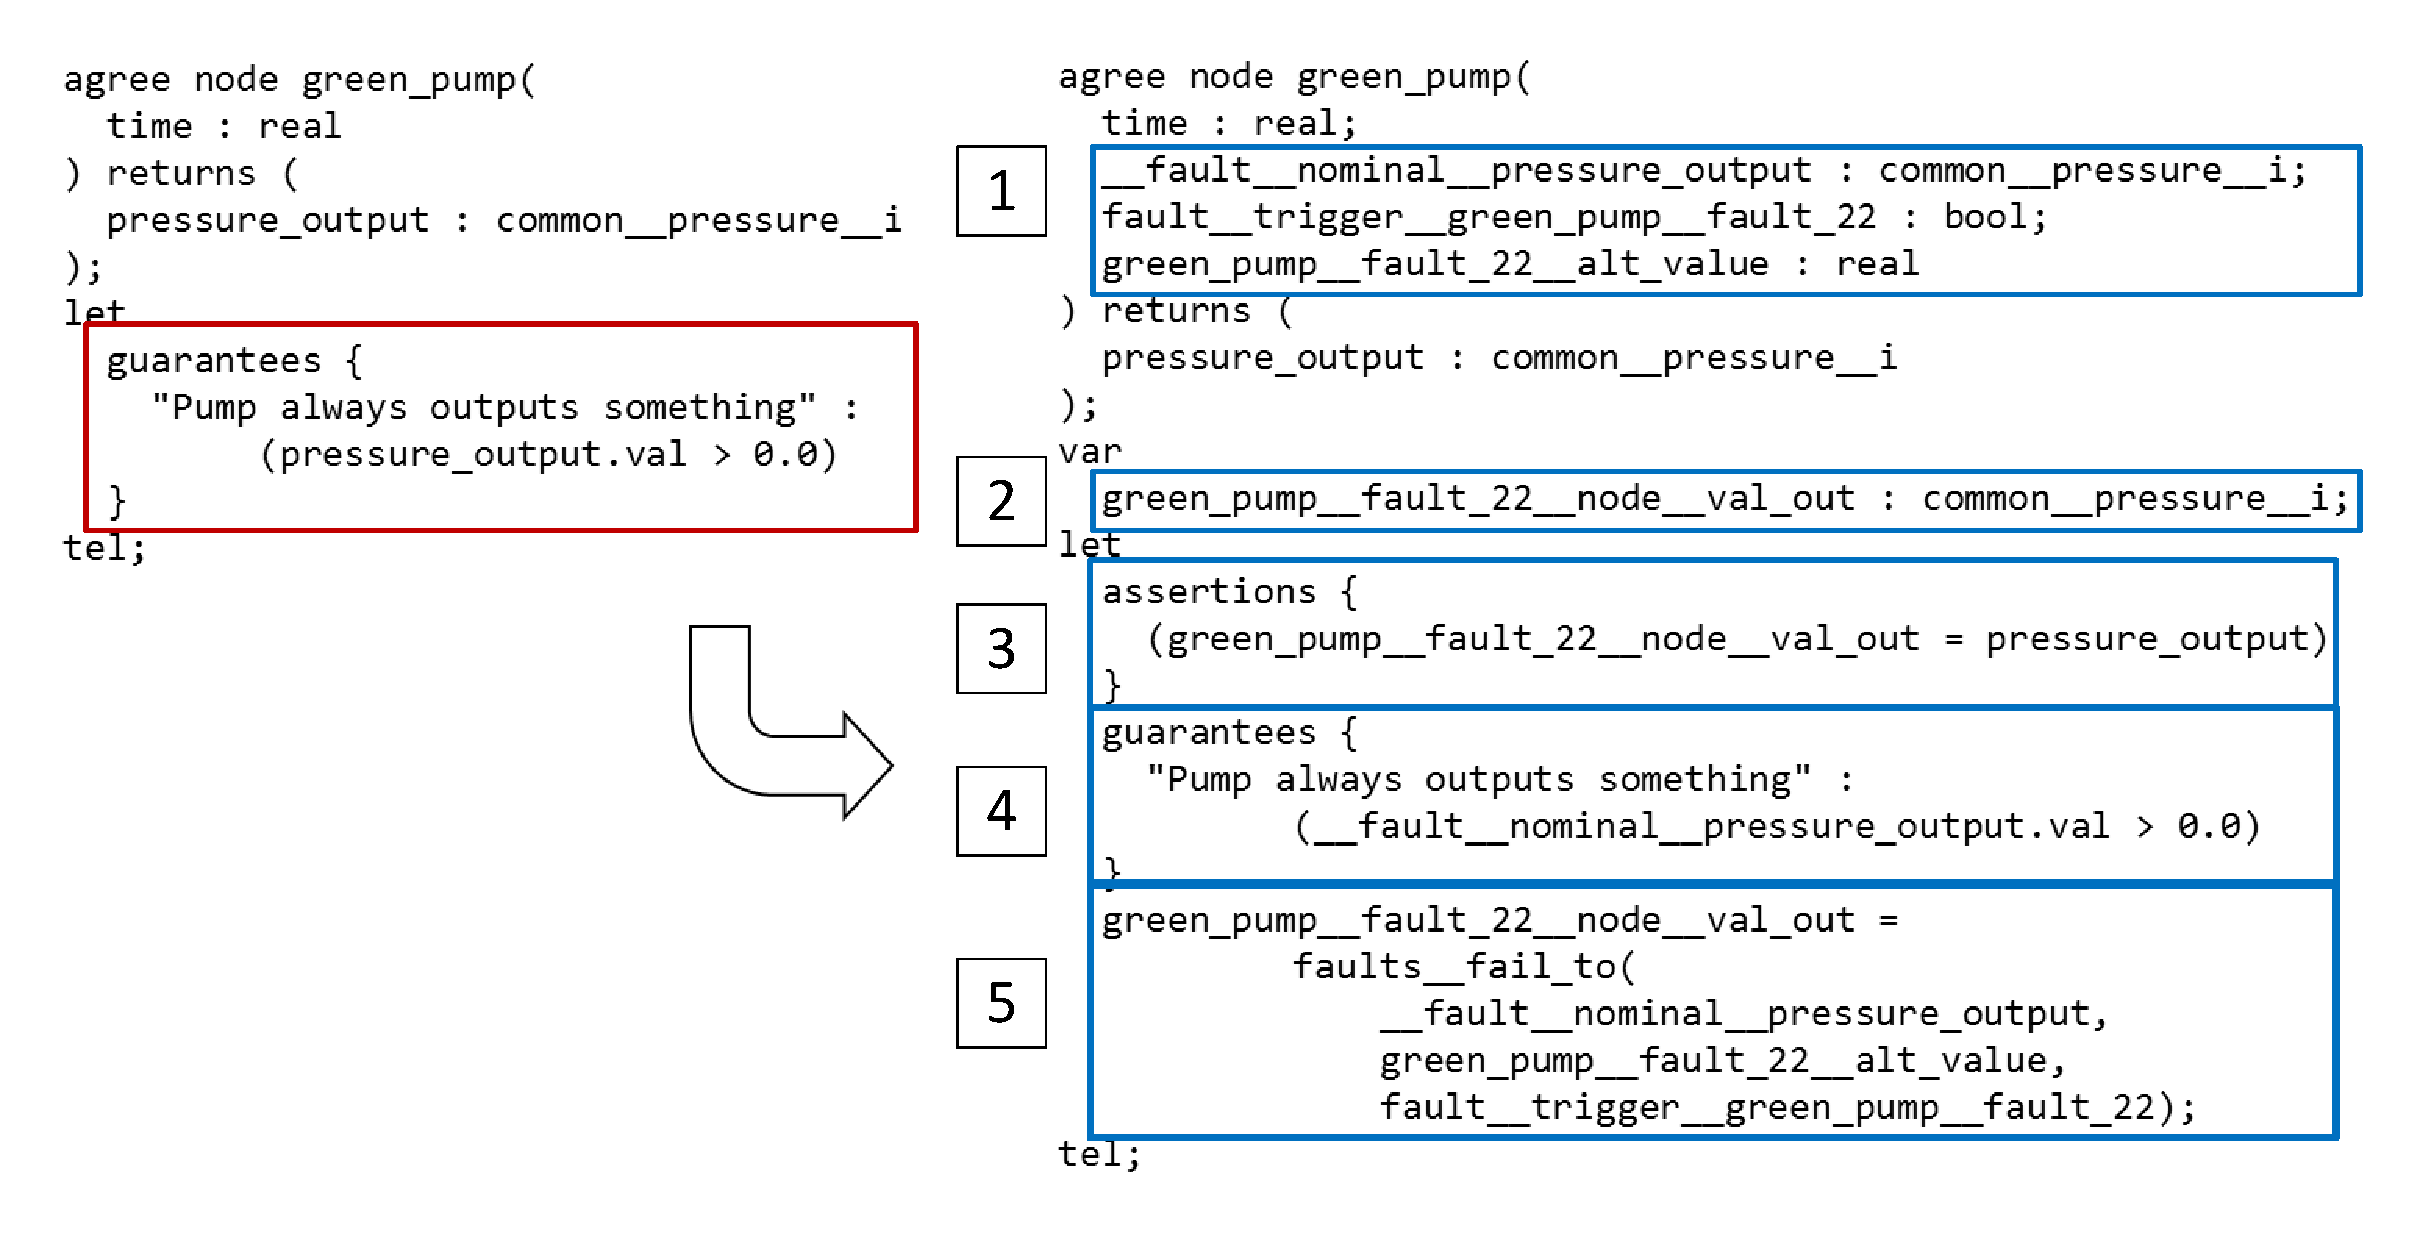
\includegraphics[trim=0 690 -10 70,clip,width=1.5\dimexpr\textwidth-2cm\relax]{images/lustre.pdf}
		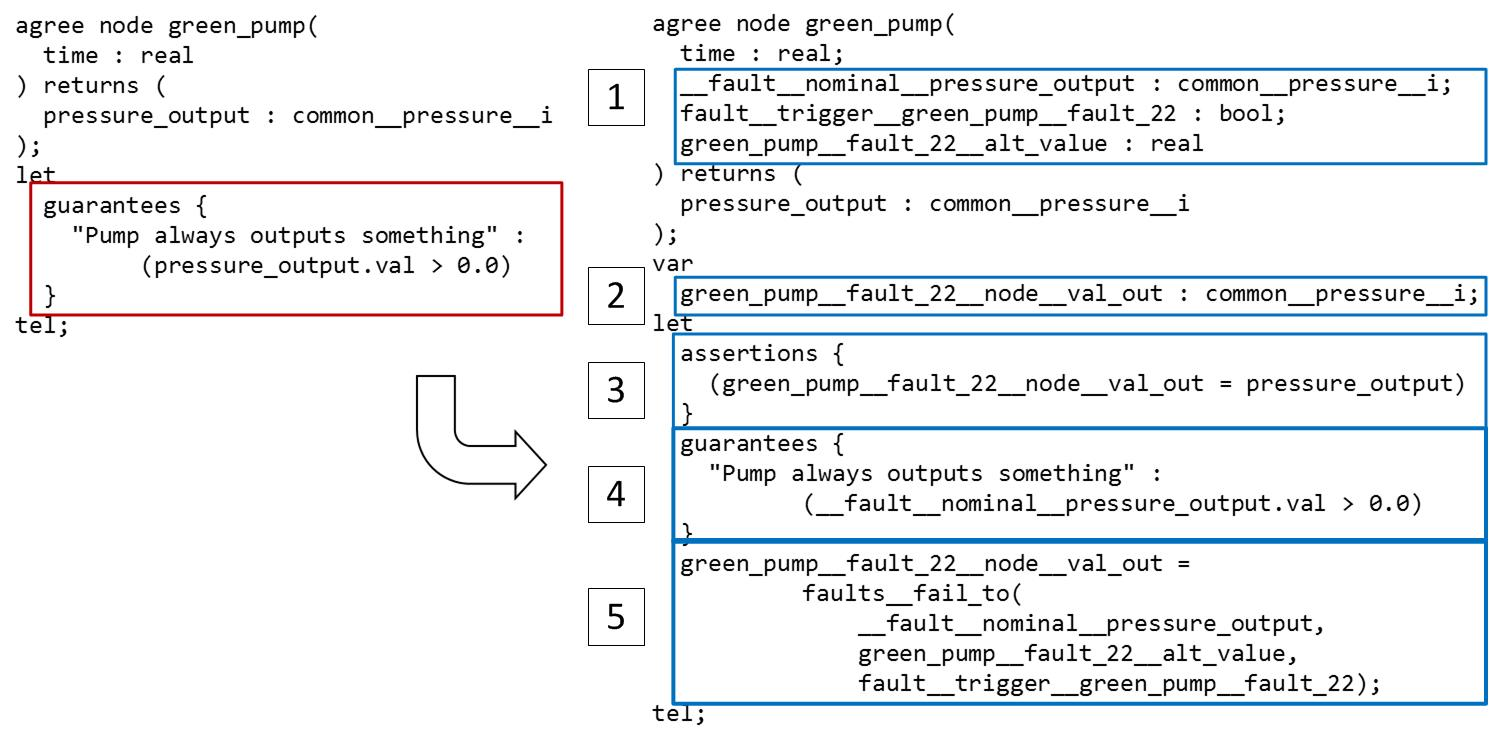
\includegraphics[scale=0.3]{images/lustre.jpg}
		\caption{Injection of Faults into Lustre Code}
		\label{fig:lustre}
	\end{center}
	\vspace{-0.3in}
\end{figure}

For fault analysis, we separate the possible analyses available to users into two distinct actions and describe them here.

\subsection{Monolithic Analysis}
When monolithic analysis is performed on the nominal system model, the architectural model is flattened in order to perform the analysis. All of the contracts in the lower levels are used for the analysis. In order to perform probabilistic fault analysis, monolithic analysis is required. A top level threshold is defined within the safety annex located in the top level system implementation. In the lower levels, each defined subcomponent fault is given a probability of occurrence. To perform this analysis, it is assumed that the non-hardware faults occur independently and possible combinations of faults are analyzed by the model checker. This corresponds to performing a prior analysis on which combinations of faults have a probability less than the threshold and then inserting assertions into the Lustre code accordingly. If the probability of such combination of faults is in fact less than the designated top level threshold, these faults may be activated and the behavioral effects can be seen through a counterexample.  

\begin{algorithm}[H]
% \KwData{this text}
% \KwResult{how to write algorithm with \LaTeX2e }
 $\mathcal{F} = \{\}$ : fault combinations above threshold \;
 $\mathcal{Q}$ : faults, $q_i$, arranged with probability high to low \;
 $\mathcal{R} = \mathcal{Q}$ , with $r \in \mathcal{R}$\;
 \While{$\mathcal{Q} \neq \{\} \land \mathcal{R} \neq \{\}$ }{
   $q =$ removePriorityElement($\mathcal{Q}$) \;
   \For{$i=0:|\mathcal{R}|$}{
       $prob = q \times r_i$ \;
       \eIf{prob $<$ threshold}{
         removeTail($\mathcal{R}, j=i:|\mathcal{R}|$)\;
       }{
        add($\{q, r_i\}, \mathcal{Q}$)\;
        add($\{q, r_i\}, \mathcal{F}$)\;
      } % end if else
   } % end for
 } % end while
 \caption{Monolithic Probability Analysis}
\end{algorithm}

The algorithm first removes all faults from consideration that are too unlikely given the probability threshold. The remaining faults are arranged in a priority queue $\mathcal{Q}$ from high to low. Assuming independence in the set of faults, we take a fault with highest probability from the queue (step 5) and attempt to combine the remainder of the faults in $\mathcal{R}$ (step 7). If this combination is lower than the threshold (step 8), then we do not take into consideration this set of faults and instead remove the tail of the remaining faults in $\mathcal{R}$. The reason we can do this is because of the arrangement in priority queue from highest to lowest value. If this combination is below threshold, certainly any other combination of these faults with one of lesser value in the priority queue will also be below threshold. 
 
In this calculation, we assume independence among the faults, but in the Safety Annex, it is possible to define dependence between faults using a \textit{hardware fault} node. At the end of Algorithm 1, the possible fault combinations reside in the list $\mathcal{F}$. We then look at the collection of propagation statements used in HW fault definitions. These have a source (HW fault) and destination (faults triggered by HW fault). 

Let $\mathcal{P}$ be the collection of propagation statements. For all $S \subset \mathcal{F}$, check to see if for $f \in S$, $f \in \mathcal{P}$ as a source. If so, add the corresponding destinations to the set $S$. This set $\mathcal{F}$ of allowed fault combinations is then added as a constraint to the Lustre model and thus they become active. 

\subsection{Compositional Analysis}
In compositional analysis, the analysis proceeds in a top down fashion. To prove the top level properties, the properties in the layer directly beneath the top level are used to perform the proof. The analysis proceeds in this manner.

 Users can constrain the maximum number of faults within each layer of the model by specifying the maximum fault hypothesis statement to that layer. If any lower level property failed due to activation of faults, the property verifications at the higher level can no longer be trusted as the higher level properties were proved based on the facts that its direct sub level properties are valid.
 
 This type of analysis is helpful to see weaknesses in a given component or layer of the system. In future work, we plan to reflect lower level property violations in the verification results of higher layers in the architecture, and enable displaying or constraining active faults system wide instead of component wide.


